\documentclass{article}
\usepackage[utf8]{inputenc}
\usepackage{pgfplots}
\pgfplotsset{width=10cm,compat=1.9}
\usepackage{amsmath,amssymb,amsthm}
\usepackage{graphicx}
\usepackage{float}
\usepackage{blindtext}
\usepackage{hyperref}
\usepackage{verbatim}
\usepackage{gensymb}
\usepackage{enumerate}
\usepackage{xcolor}
\usepackage{graphicx}
\hypersetup{
    colorlinks=true,
    linkcolor=blue,
    filecolor=magenta,      
    urlcolor=cyan,
    pdftitle={Overleaf Example},
    pdfpagemode=FullScreen,
    }
\usepackage[slovene]{babel}

\setlength{\parindent}{0pt}
\setlength{\parskip}{4pt}

\newcommand{\Lim}[1]{\raisebox{0.5ex}{\scalebox{0.8}{$\displaystyle \lim_{#1}\;$}}}
\newcounter{example}[section]
\newenvironment{example}[1][]{\refstepcounter{example}\par\medskip
   \noindent \textbf{Naloga~\theexample. #1} \rmfamily}{\medskip}

\newtheorem*{zgled}{Zgled}

\title{Funkcije}
\author{Bor Bregant}
\date{\vspace{-5ex}}

\begin{document}

\maketitle

Funkcija ali preslikava $f$ iz množice $A$ v množico $B$ je predpis, ki vsakemu elementu iz $A$ priredi natanko en element iz množice $B$.

\begin{zgled}
    Zapiši definicijsko območje in ničle za funkcijo $f(x)=\sqrt{x^2-1}$ in $g(x)=\log{\left(x(x-1)(x+1)\right)}$. Ob grafu funkcije zapiši zalogo vrednosti intervale naraščanja in obravnavaj konveksnost za $h(x) = \cos\left(x-\frac{\pi}{2}\right)-4$. Obravnavaj sodost / lihost za $f(x)=x^2 +x^6$ in $g(x)=x+x^3$.
\end{zgled}

\section{Računanje s funkcijami}

\begin{enumerate}[i]
    \item Vsota $\left(f+g\right)(x)=f(x)+g(x)$
    \item Razlika $\left(f-g\right)(x)=f(x)-g(x)$
    \item Produkt $\left(f\cdot g\right)(x)=f(x)\cdot g(x)$
    \item Kvocient $\left(\frac{f}{g}\right)(x)=\frac{f(x)}{g(x)}$ za $g(x)\neq 0, \forall x\in D_g$
    \item Produkt s številom $\left(k\cdot f\right)(x)=k \cdot f(x)$
\end{enumerate}

\begin{zgled}
    Zapiši vsoto, razliko, produkt in kvocient funkcij $f(x)=x-3$ in $g(x)=-2x+1$.
\end{zgled}

\begin{example}
    DN 569c, 576, 578ad
\end{example}

\subsection*{Kompozitum funkcij}

\begin{figure}[H]
    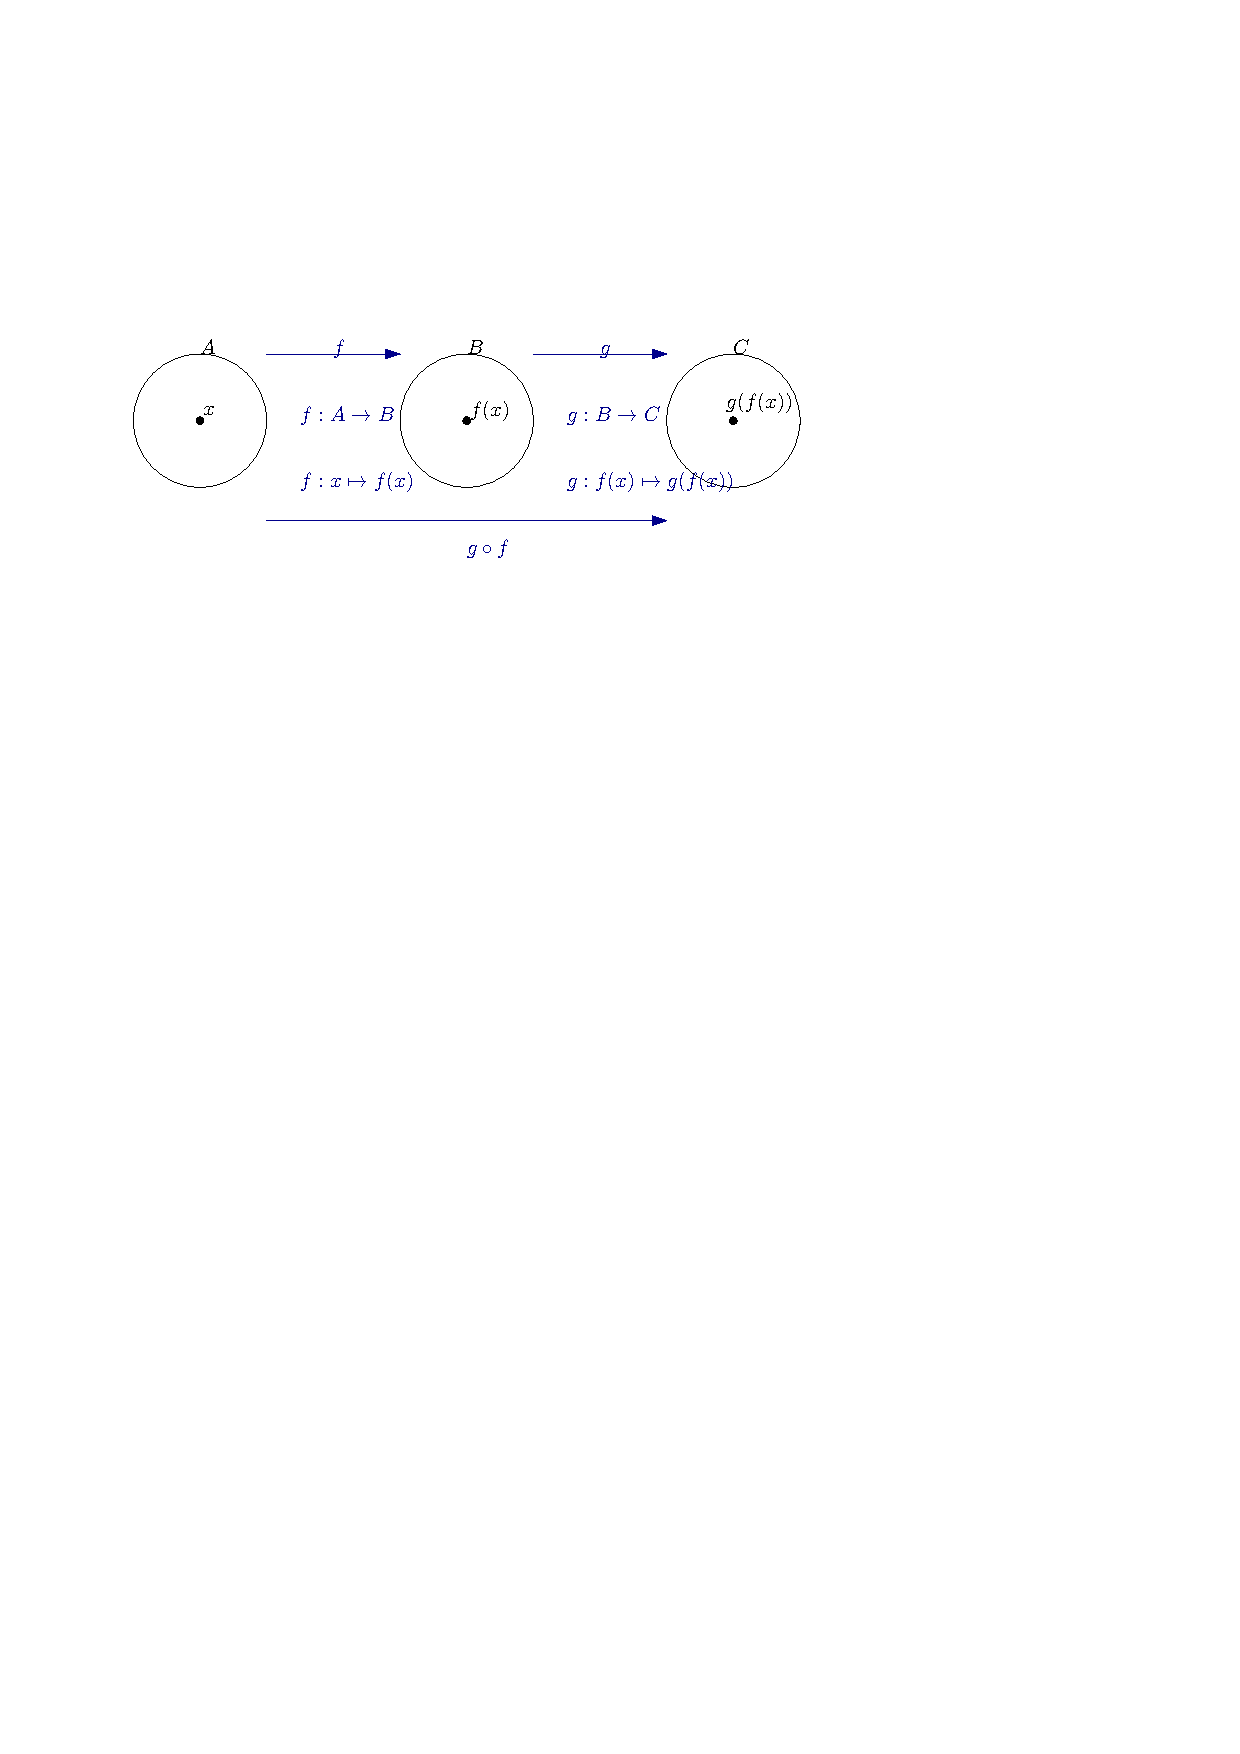
\includegraphics[width=0.7\textwidth]{kompozitum.pdf}
    \centering
\end{figure}

\begin{align*}
    & g\circ f: A\rightarrow C\\
    & g\circ f: x\mapsto g(f(x))\\
    & (g\circ f)(x)=g(f(x))\\
\end{align*}

\begin{zgled}
    Izračunaj $f\circ g$ in $g\circ f$ za $f(x)=\ln (x^2+2)$ in $g(x)=3x-1$ in pokaži, da ta operacija ni komutativna.
\end{zgled}

\begin{zgled}
    Poišči inverzno funkcijo za $f(x)=\sqrt[3]{x}+1$ in pokaži, da velja $(f\circ f^{-1})(x)=(f^{-1}\circ f)(x)=x$.
\end{zgled}
   
\begin{zgled}
    Dani sta funkciji $f(x)=2x-3$ in $g(x)=-x+2$. Za katera realna števila $x$ je $f(2x)=g(x)$ in za katera $f(-2)=g(x^2)$.
\end{zgled}

\begin{zgled}
    Dani sta funkciji $f(x)=3x+2$ in $g(x)=2x+n$. Za katera števila $n$ velja $f(g(x))=g(f(x))$?
\end{zgled}

\begin{zgled}
    Določi $k$, da bo $f(g(x))=g(f(x))$, kjer $f(x)=kx+3$ in $g(x)=kx-1$.
\end{zgled}

\begin{example}
    DN 574, 573ace, 587, 592ac
\end{example}

\section*{Limita in zveznost}

\subsection*{Zveznost}

\begin{zgled}
    Narišimo funkcije
    \begin{align*}
        &f(x) = 
             \begin{cases}
               2 & x>0\\
               0 &x=0 \\
               -x-1 &x<0\\
             \end{cases}\\
        &g(x) = 
             \begin{cases}
               |x+1| & x\neq 0\\
               0 &x=0\\
             \end{cases}\\
        &h(x) = 
             \begin{cases}
               x+1 & x\leq 0\\
               e^x &x>0\\
             \end{cases}\\
    \end{align*}
    Opazimo, da $f$ in $g$ ista zvezni v $x=0$, ampak lahko $g$ popravimo v zvezno če dopolnimo z $1$. $h$ je zvezna. $g$ ima v $x=0$ limito, $f$ pa ne.
\end{zgled}

Funkcije, ki lahko narišemo z eno potezo so \textbf{zvezne}, sicer pa \textbf{nezvezne}.

Funkcija $f$ je zvezna v točki $a$, če in samo če:
\[\forall \varepsilon >0 \exists \delta >0: |x-a|<\delta \Rightarrow |f(x)-f(a)|<\varepsilon\]

$f$ je zvezna na $[a,b]$, če je zvezna v vsaki točki tega intervala. Vse elementarne funkcije so zvezne, kjer so definirane.


\begin{zgled}
    Nariši graf
    \begin{align*}
        &f(x) = 
             \begin{cases}
               2^x & x\leq 0\\
               x^{-1} &0<x<1 \\
               2x-1 &x\geq 1\\
             \end{cases}\\
        &g(x) = 
             \begin{cases}
               \sin x & x\leq 0\\
               \tan x &x>0\\
             \end{cases}\\
    \end{align*}
    in zapiši točke nezveznosti.
\end{zgled}

\begin{zgled}
    Določi $a\in\mathbb{R}$, da bo funkcija
    $f(x) = 
             \begin{cases}
               x^2 & x > 4\\
               x+a & x\leq 4 \\
             \end{cases}$
    zvezna.
\end{zgled}

\begin{example}
    DN 597bčef, 598abc
\end{example}

\subsection*{Limita}

\begin{zgled}
    Nariši $f(x)=\tan x$ in $g(x)=\frac{x+1}{(x-1)^2}$ in opazuj točke nedefiniranosti.

    Enako za $f(x) = 
             \begin{cases}
               x+2 & x < -1\\
               -1 & x \geq -1 \\
             \end{cases}$.
\end{zgled}

Limita je neke vrste nadomestek za vrednost funkcije.

\[b=\lim_{x\rightarrow a}f(x) \iff \forall \varepsilon >0 \exists \delta >0: |x-a|<\delta \Rightarrow |f(x)-b|<\varepsilon\]

Število $b$ je limita funkcije $f$, ko gre $x$  proti $a$, če za poljubno $\varepsilon$ okolico točke $b$ obstaja taka $\delta$ okolica točke $a$, da brž ko je $x$ v $\delta$ okolici točke $a$, je tudi $f(x)$ v $\varepsilon$ okolici točke $b$.

\begin{figure}[H]
    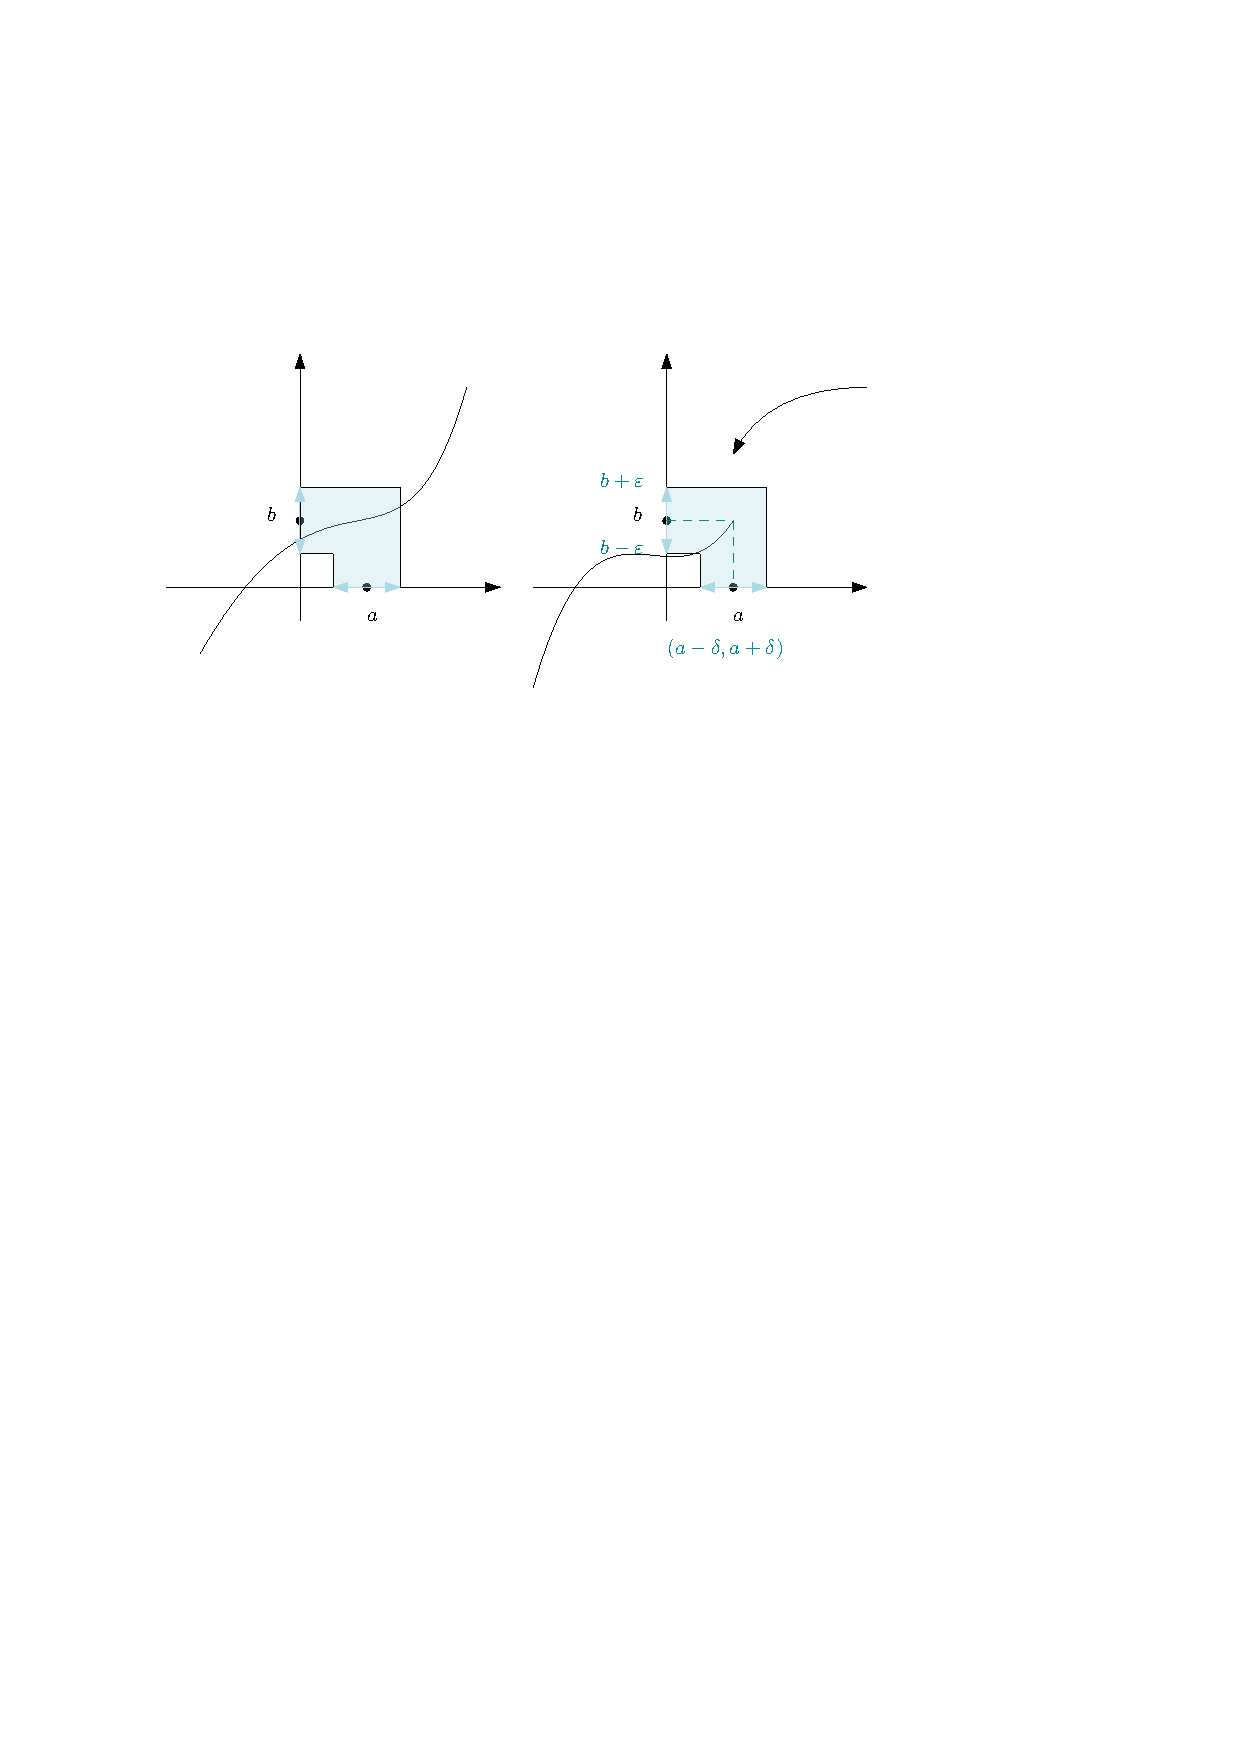
\includegraphics[width=0.8\textwidth]{limite_def.pdf}
    \centering
\end{figure}

\begin{zgled}
    Izračunaj $\Lim{x\rightarrow -1} (2x^2+x)$, $\Lim{x\rightarrow \frac{1}{2}} \frac{\log_2 x}{4^x}$ in $\Lim{x\rightarrow 2} \frac{x^2-7x+10}{x^2-4}$.
\end{zgled}

\begin{zgled}
    Izračunaj $\Lim{x\rightarrow 0}\frac{\sqrt{x^2 +100}-10}{x^2}$. \textcolor{gray}{korenska limita}
\end{zgled}

\begin{example}
    DN 606bč, 607bdc, 608c, 624bč
\end{example}

\subsubsection*{Limita v neskončnosti in neskončna limita}

\[\Lim{x\rightarrow a}=\infty \iff \forall M\in\mathbb{R} \exists \delta >0: |x-a|<\delta \Rightarrow f(x)>M\]

\begin{zgled}
    Izračunaj $\Lim{x\rightarrow 0} \frac{1}{x}$, $\Lim{x\rightarrow 0} \frac{1}{x^2}$ in $\Lim{x\rightarrow 2} \frac{x-1}{\left(x+2\right)^2}$.
\end{zgled}

\[b=\Lim{x\rightarrow\infty}\iff \forall \varepsilon >0 \exists M\in \mathbb{R}: x>M \Rightarrow |f(x)-b|<\varepsilon\]

\begin{zgled}
    Izračunaj $\Lim{x\rightarrow \pm \infty} \frac{1}{x}$, $\Lim{x\rightarrow \infty} \arctan x + 1$ in $\Lim{x\rightarrow \pm \infty} 3^{-x + 2}$.
\end{zgled}

\begin{example}
    DN 614d, 615ac, 619cč
\end{example}

\subsection*{Pravila za računanje z limitami}

\begin{enumerate}[i]
    \item $\Lim{x\rightarrow a}\left(f(x)\pm g(x)\right)=\Lim{x\rightarrow a} f(x)\pm \Lim{x\rightarrow a} g(x)$
    \item $\Lim{x\rightarrow a} kf(x)=k\Lim{x\rightarrow a}f(x)$
    \item $\Lim{x\rightarrow a}\left(f(x)\cdot g(x)\right)=\Lim{x\rightarrow a} f(x)\cdot \Lim{x\rightarrow a} g(x)$
    \item Enako za kvocient, potenco, koren
    \item $\Lim{x\rightarrow a}c=c$
\end{enumerate}

\subsubsection*{Limita $e$ in $\frac{\sin x}{x}$}

\[\Lim{x\rightarrow\infty}\left(1+\frac{1}{x}\right)^x =e\]

\[\Lim{x\rightarrow 0} \frac{\sin x}{x} =1\]

\begin{zgled}
    Izračunaj lazji?, $\Lim{x\rightarrow\infty}\left(\frac{5x+3}{5x-7}\right)^x$ in $\Lim{x\rightarrow\infty}\left(\frac{3x-1}{x+2}\right)^x$ in $\Lim{x\rightarrow\infty}\left(\frac{x+2}{x+5}\right)^{x+1}$
\end{zgled}

\begin{example}
    DN 625bc
\end{example}

\begin{zgled}
    Izračunaj $\Lim{x\rightarrow 0}\frac{\sin 3x}{2x}$, $\Lim{x\rightarrow 0}\frac{\sin 3x}{\sin 4x}$, $\Lim{x\rightarrow 0}\frac{1-\cos x}{x}$ \textcolor{gray}{razširimo s konjugirano} in $\Lim{x\rightarrow 0} x^{-1}\tan x \cos x$.
\end{zgled}

\begin{example}
    DN 621acče, 623č\textcolor{red}{e}, 626c
\end{example}


\end{document}